\documentclass[border=2pt]{standalone}
\usepackage{tikz}
\usetikzlibrary{calc} \usetikzlibrary{positioning} \usetikzlibrary{shapes,arrows} \usetikzlibrary{plotmarks}
\usepackage{pgfplots}
\usetikzlibrary{patterns}

\begin{document}

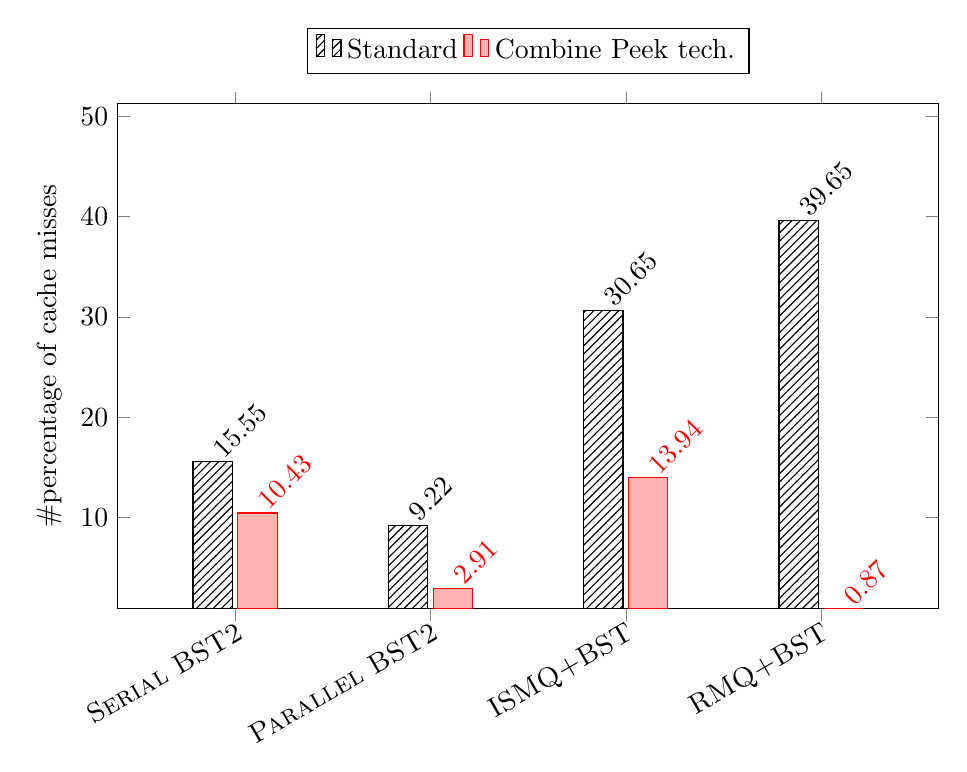
\begin{tikzpicture}
  \centering
  \begin{axis}[
    bar width=0.5cm,
    ybar,
    xtick=\empty,
    enlargelimits=0.20,
    legend style={at={(0.5,1.15)},
    anchor=north,legend columns=-2},
    ylabel={\#percentage of cache misses},
    symbolic x coords={Serial BST2,Parallel BST2, ISMQ+BST, RMQ+BST},
    xtick={Serial BST2,Parallel BST2, ISMQ+BST, RMQ+BST},
    height=8cm,width=12cm,
    nodes near coords,
    nodes near coords align={vertical},
    every node near coord/.append style={
        anchor=mid west,
        rotate=45
    },
    xticklabel style={
        inner sep=0pt,
        anchor=north east,
        rotate=30,
        font=\scshape,
    },
    enlarge y limits={upper,value=0.3},
    ]
    \addplot[pattern=north east lines] coordinates 
        {(Serial BST2,15.546)  (Parallel BST2,9.218)
         (ISMQ+BST,30.649) (RMQ+BST,39.652)
        };
    \addplot coordinates 
        {(Serial BST2,10.430)  (Parallel BST2,2.914)
         (ISMQ+BST,13.936) (RMQ+BST,0.871)
        };
    \legend{Standard, Combine Peek tech.};
  \end{axis}
\end{tikzpicture}

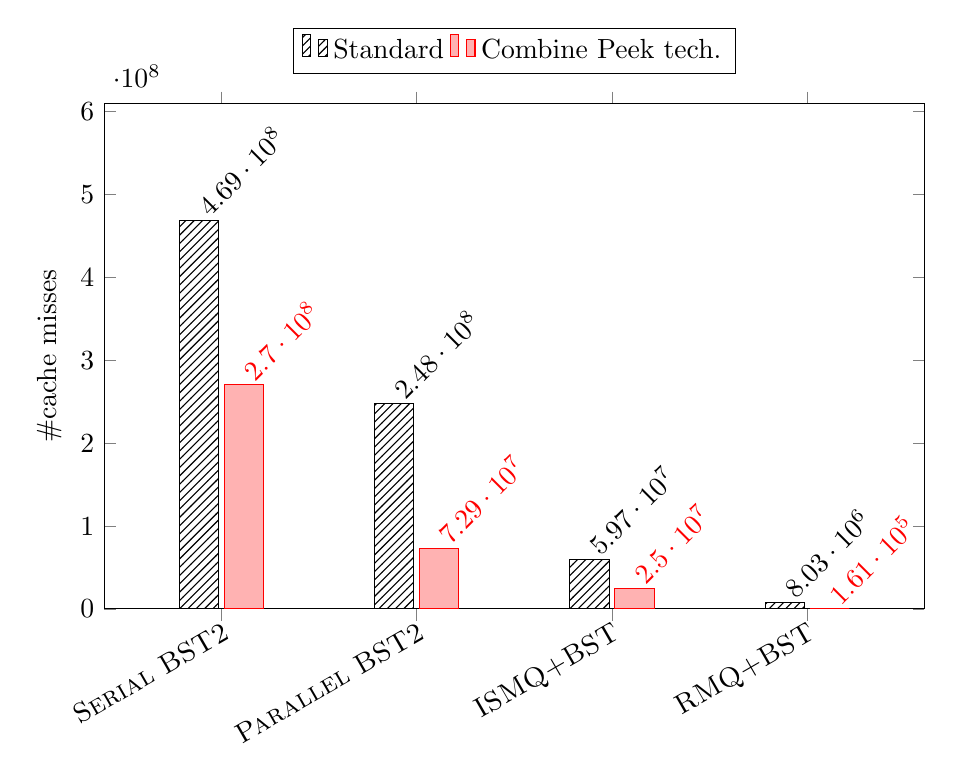
\begin{tikzpicture}
  \centering
  \begin{axis}[
    bar width=0.5cm,
    ybar,
    xtick=\empty,
    enlargelimits=0.20,
    legend style={at={(0.5,1.15)},
    anchor=north,legend columns=-2},
    ylabel={\#cache misses},
    symbolic x coords={Serial BST2,Parallel BST2, ISMQ+BST, RMQ+BST},
    xtick={Serial BST2,Parallel BST2, ISMQ+BST, RMQ+BST},
    height=8cm,width=12cm,
    nodes near coords,
    nodes near coords align={vertical},
    every node near coord/.append style={
        anchor=mid west,
        rotate=45
    },
    xticklabel style={
        inner sep=0pt,
        anchor=north east,
        rotate=30,
        font=\scshape,
    },
    enlarge y limits={upper,value=0.3},
    ]
    \addplot[pattern=north east lines] coordinates 
        {(Serial BST2,469079337)  (Parallel BST2,247734674)
         (ISMQ+BST,59693500) (RMQ+BST,8028026)
        };
    \addplot coordinates 
        {(Serial BST2,270465307)  (Parallel BST2,72918082)
         (ISMQ+BST,24954642) (RMQ+BST,161066)
        };
    \legend{Standard, Combine Peek tech.};
  \end{axis}
\end{tikzpicture}


\end{document}